\documentclass[a4paper,10pt]{report}
\usepackage[utf8]{inputenc}
\usepackage{graphicx}
\usepackage{subcaption}
\usepackage{parskip}
\usepackage{amsmath}
\usepackage{listings}
\usepackage{color}
\usepackage{listings}

\definecolor{red}{rgb}{1,0,0}
\definecolor{green}{rgb}{0,1,0}
\definecolor{codegreen}{rgb}{0,0.6,0}
\definecolor{codegray}{rgb}{0.5,0.5,0.5}
\definecolor{codepurple}{rgb}{0.58,0,0.82}
\definecolor{backcolour}{rgb}{0.95,0.95,0.92}

\lstdefinestyle{mystyle}{
    backgroundcolor=\color{backcolour},   
    commentstyle=\color{blue},
    numberstyle=\tiny\color{codepurple},
    stringstyle=\color{codegreen},
    basicstyle=\footnotesize,
    breakatwhitespace=false,         
    breaklines=true,                 
    captionpos=b,                    
    keepspaces=true,                 
    numbers=left,                    
    numbersep=5pt,                  
    showspaces=false,                
    showstringspaces=false,
    showtabs=false,                  
    tabsize=2
}
 
\lstset{style=mystyle,language = C}

%opening
\title{LIC, UNIK4660 Obligatory Assignment}
\author{Joseph Knutson}

\begin{document}

\maketitle
\section*{Introduction}
The aim of this assignment is to present geometric and texture based visualization methods for visualizing 2D vector field data. The geometric method is composed of the visualization of streamlines produced from numerical integration of the velocity field.
The texture based method used is LIC, proposed by Brian Cabral and Leith Leedom\footnote[1]{Cabral, Brian; Leedom, Leith Casey (August 2–6, 1993). "Imaging Vector Fields Using Line Integral Convolution"}. Finally, we will compare the resulting imagery.


\section*{Data}
To start off with, the 2 vector field data files we're looking at has different, but quadratic resolutions. The set called "metsim1" is 127 by 127, while the one called "isabel" is 500 by 500. In order to increase the resolution, I've implemented a simple interpolator which increases the resolution by any order of 2.

The datasets are stored in the HDF5 format as 1D arrays. In order to extract the vector-field data, we need to use the HDF5 library, written in, but perhaps not exclusively for, PYTHON and C/C++.
For this assignment I'll be using C++ for the integration and texture visualization and PYTHON(2.7) for the geometric visualization.

\subsection*{HDF5}

Below is a function that extracts the vector field data to the 1D vectors "rdata" and "rdata2":
\begin{lstlisting}
void 
init(hid_t file, hid_t dset,hid_t dset2, herr_t status,herr_t status2,double* rdata,double* rdata2){

      file = H5Fopen (FILE, H5F_ACC_RDONLY, H5P_DEFAULT);
      dset = H5Dopen (file, DATASET, H5P_DEFAULT);
      dset2 = H5Dopen (file, DATASET2, H5P_DEFAULT);

      status = H5Dread (dset, H5T_NATIVE_DOUBLE, H5S_ALL, H5S_ALL, H5P_DEFAULT,rdata);
      status2 = H5Dread (dset2, H5T_NATIVE_DOUBLE, H5S_ALL, H5S_ALL, H5P_DEFAULT,rdata2);
    }
\end{lstlisting}
First the function opens the file whose name is stored as a string in the "FILE" variable.
It then splits the dataset into its x and y sub-datasets seperately. These datasets are then "read", or rather inserted, into the rdata arrays thanks to the H5Dread method from the HDF5 library.
\section*{Integration and Seeding}
After extracting the vector field data, we can begin integrating streamlines.
I've implemented both the forward Euler and 4th order Runge Kutta method. The timestep seems to be optimal around the value 1, causing the streamlines to jump to its neighbouring pixel. This might be due to the velocity normalization.
The Euler and RK4 method seem to not give different results visualization-wise. I believe this is due to the extreme discreteness of our data/grid. A 3 times speed up is therefore achieved when keeping to the Euler method.

I've only tried 2 types of seeding, random and uniform. With random, I mean that the initial position of the streamlines have been chosen randomly throughout the grid. The uniform technique consisted of homogenously planting 
the lines' initial positions across the grid. In figure \ref{fig1} and \ref{fig2} you can observe both seeding strategies in effect. 

The homogenously distributed lines are evenly dispersed, while the random seeding has chunks of lines overlapping.
My favorite is the uniform/homogenous one, but it too has problems detailing the center and corners of the field.

Seeding isn't the only thing we can tweak, we can also experiment with line length. Figures \ref{fig3}, \ref{fig4} and \ref{fig5} show how the images can vary when the line length goes from 1/10th of the image's length to 4/10. To keep things fresh, these are from the Isabel dataset.



\begin{figure}\centering
 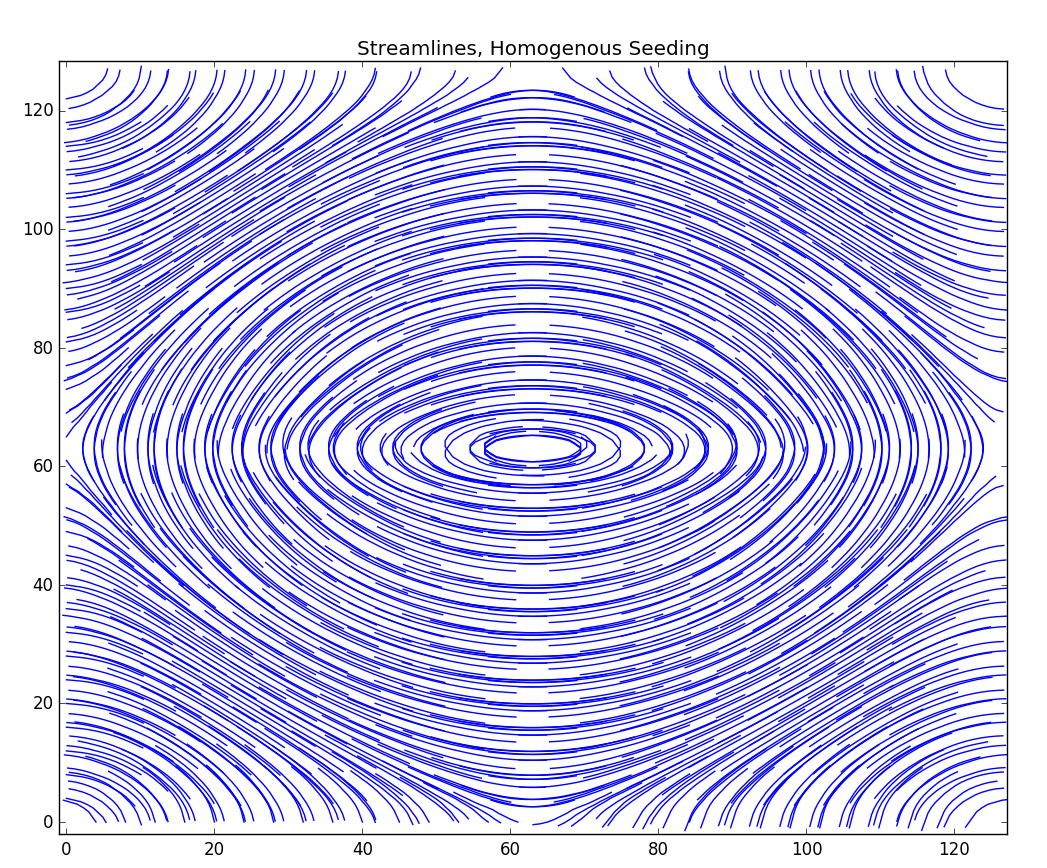
\includegraphics[width=0.9\linewidth]{homo}
 \caption{1000 streamlines from the Metsim set. The seeding is homogenously distributed through the vectorfield.}
 \label{fig1}
\end{figure}

\begin{figure}\centering
 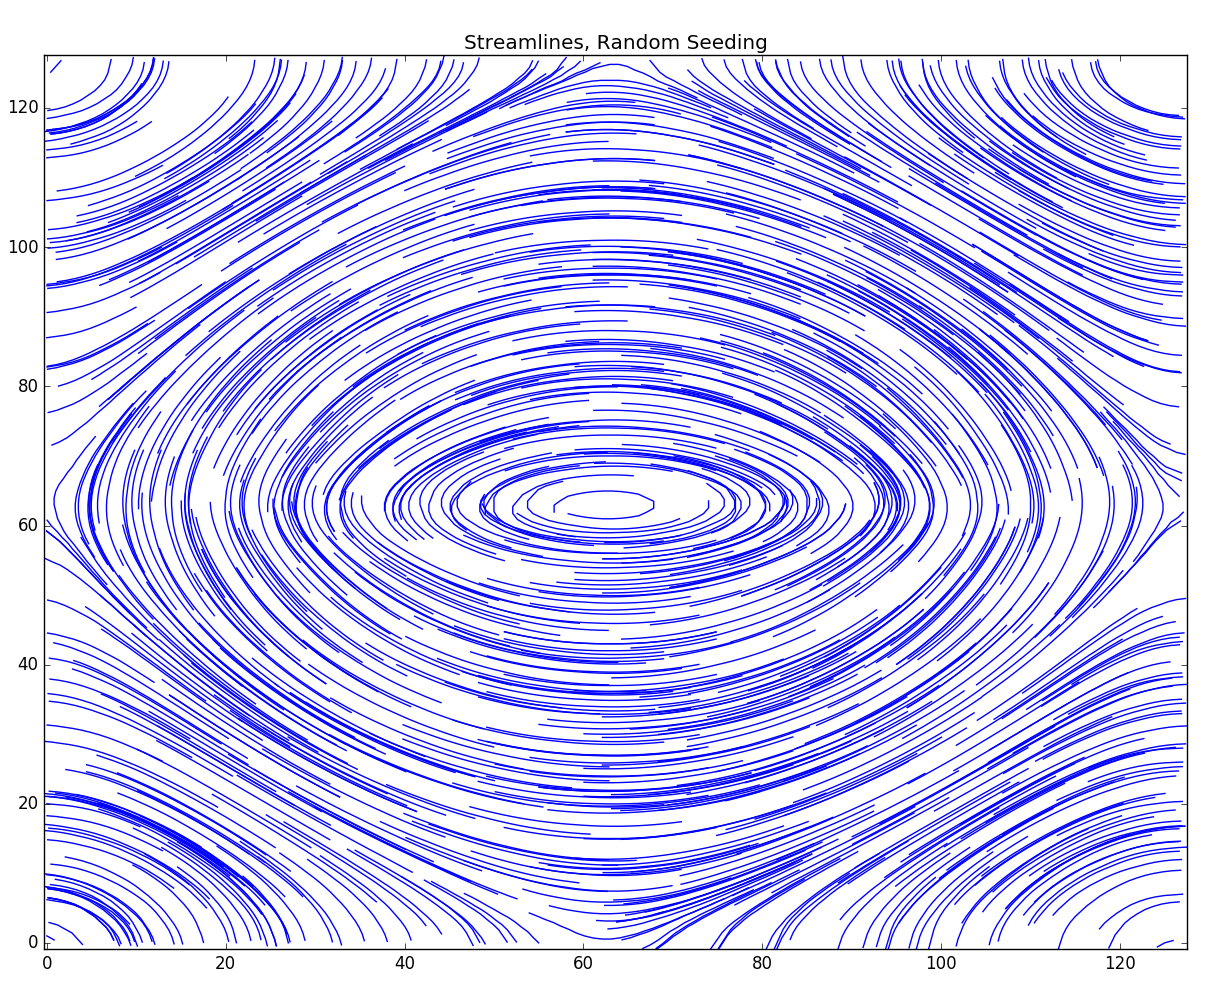
\includegraphics[width=0.9\linewidth]{random}
 \caption{This time the seeding is randomly distributed through the vectorfield.}
 \label{fig2}
\end{figure}
\clearpage
\begin{figure}\centering
 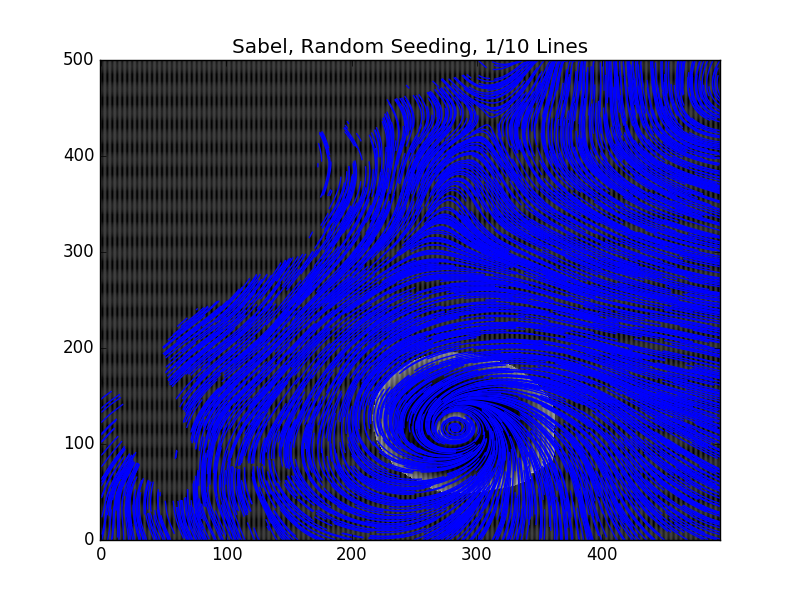
\includegraphics[width=0.9\linewidth]{short}
 \caption{The short lines' cutoffs are visible and not esthetically pleasing.}
 \label{fig3}
\end{figure}

\begin{figure}\centering
 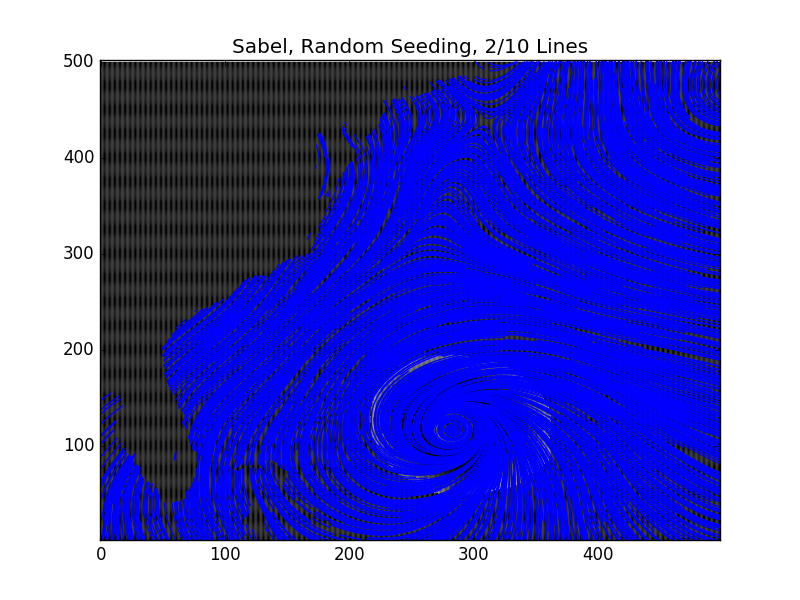
\includegraphics[width=0.9\linewidth]{medium}
 \caption{The medium length lines give a smoother feel, but the lines lie rather dense together.}
 \label{fig4}
\end{figure}
\begin{figure}\centering
 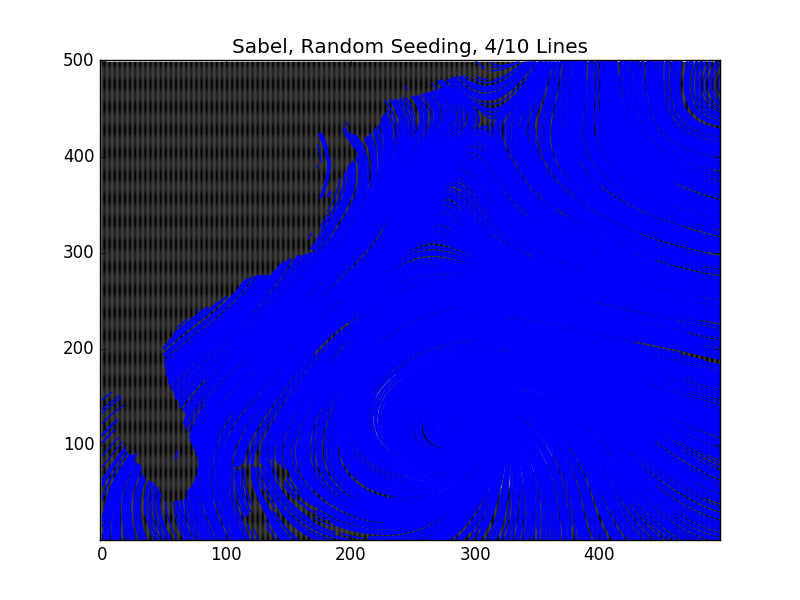
\includegraphics[width=0.9\linewidth]{long}
 \caption{Blue, blue everywhere.}
 \label{fig5}
\end{figure}
\clearpage
\section*{LIC}
The implementation of the LIC algorithm went something like this:
\begin{itemize}
 \item Superimpose your vector field over a noise filter
 \item Create streamlines, one for each pixel, more if your vectorfield grid is denser than your pixel grid.
 \item Convolve the streamlines. Do so along the noisefilter so that the weighted average intensity is produced. This is now that pixel's grey-image-value. Do this multiple times for pixels that initiate more than one streamline and take the average. 
\end{itemize}

My implementation was quite simple. I created a grey image noise filter with values between 0 and 255. Its dimensions are always the same as the vector-field and the vectorfield is interpolated to any degree I wish.
Changing the dimensions of the filter is unecessary as it has no effect on the operations. 

Below are LIC images of both datasets with increasing line lengths. You can see smoothening of the image the longer the lines, but as the image gets smoother, it also gets harder to distinguish field lines and extract information.
In contrast, shorter lines will sometimes be too short to visualize a continuing line, ruining the pattern of the field.

The increase in line length seems to cause a linear increase in processing time.
Setting the line length equal to 10\% of the image width seems to make the most prominent pattern. 

\section*{Conclusion}
When done right, LIC can beautifully render 2D veolocity fields in a much more fashionable way than streamlines alone. 
However, if you choose to visualize with streamlines alone, pure random seeding will cause ugly areas of
overlapping lines (or voids). Uniform seeding might remove the problem with overlapping lines, but due to topological complications, certain areas will become under-represented.

Euler and RK show no noticeable differences in the images, due to our low image resolution. The timestep's optimal value being 1 is 
likely due to the vector field normalization in the integration scheme.

When visualizing geometrically, too short lines will give an ugly and tacky image, while a textured image would simply be chaotically patternless.
Long lines and random seeding seem to cause streamlines to overlap to the extent that entire parts of the picture are single colored chunks.
While in LIC's case, the dynamics and directional sense of the image is lost due to long lines causing a bland, contrastless smoothness in the field. This is perhaps only visible in figure \ref{fig13}.
\clearpage
\begin{figure}\centering
 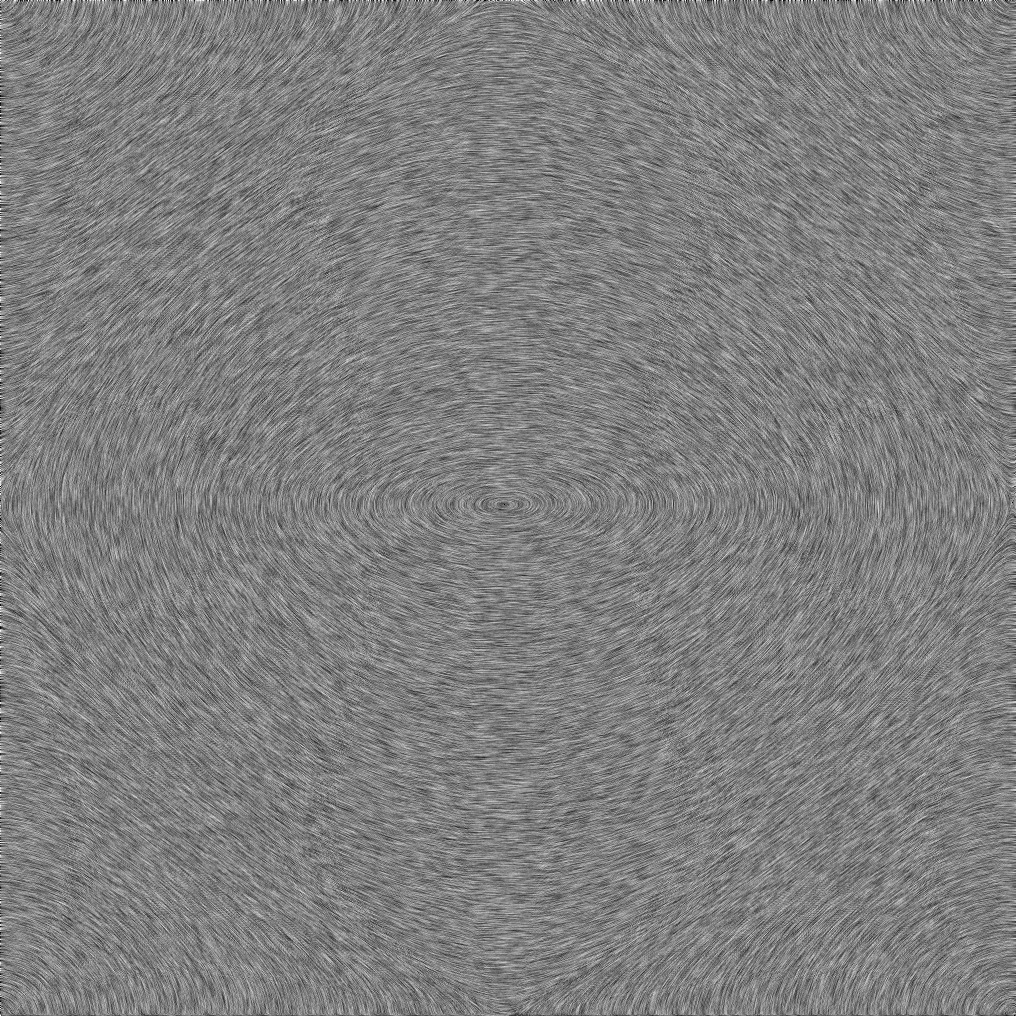
\includegraphics[width=0.7\linewidth]{metsim_linelength_5_highdef.jpg}
 \caption{Textured LIC image from streamlines whose length is 5\% of the image width or height. Quite tacky}
 \label{fig8}
\end{figure}
\begin{figure}\centering
 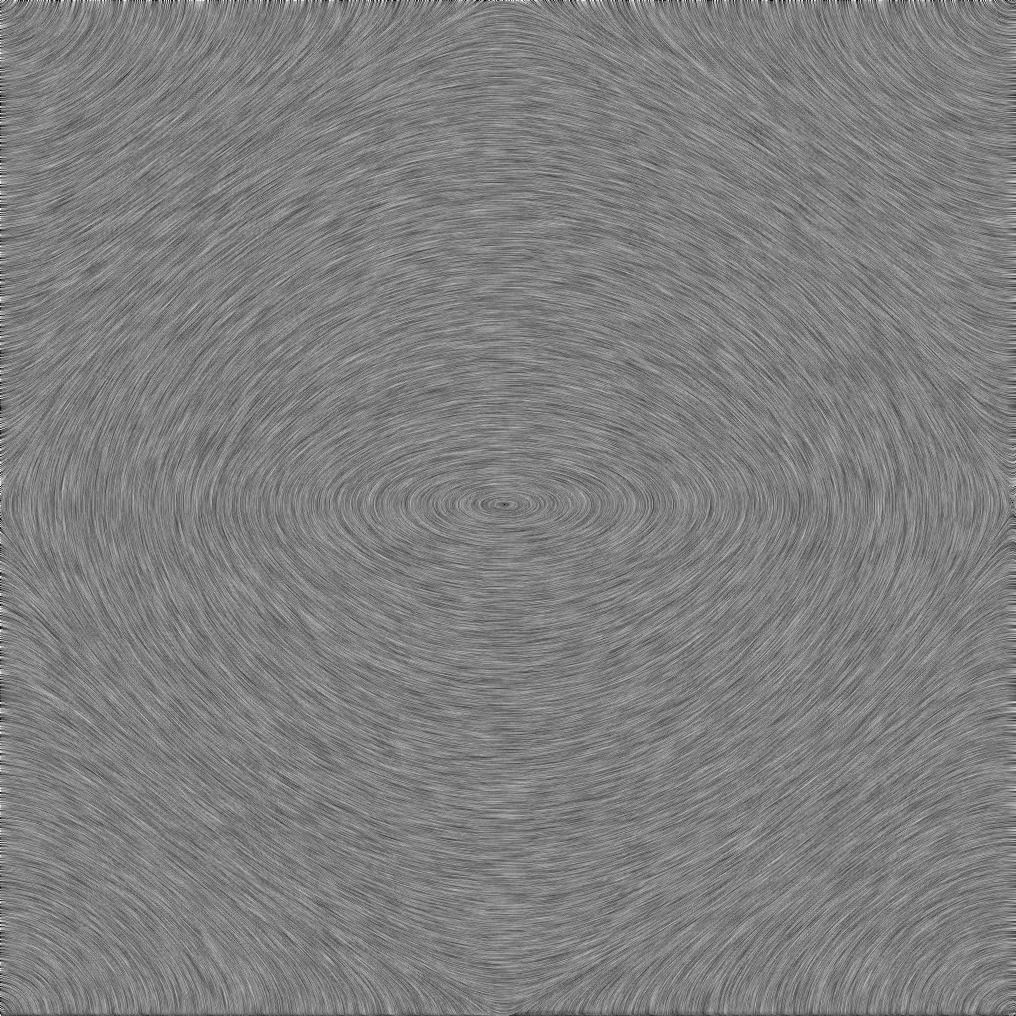
\includegraphics[width=0.7\linewidth]{metsim_linelength_10_highdef.jpg}
 \caption{Medium Lines (10\% of the image width)}
 \label{fig9}
\end{figure}
\begin{figure}\centering
 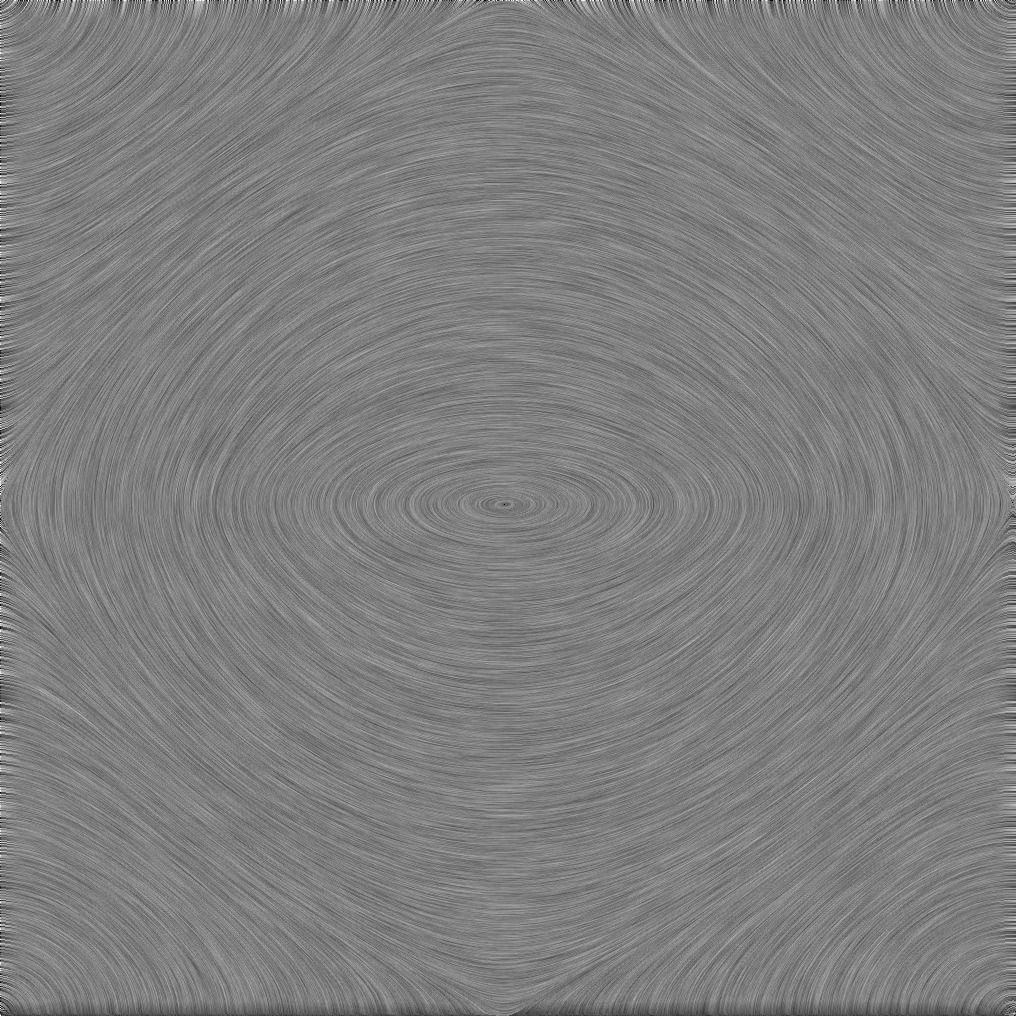
\includegraphics[width=0.7\linewidth]{metsim_linelength_20_highdef.jpg}
 \caption{Long lines, with the length of 20\% the image width seems an apt length for this resolution.}
 \label{fig10}
\end{figure}

\begin{figure}\centering
 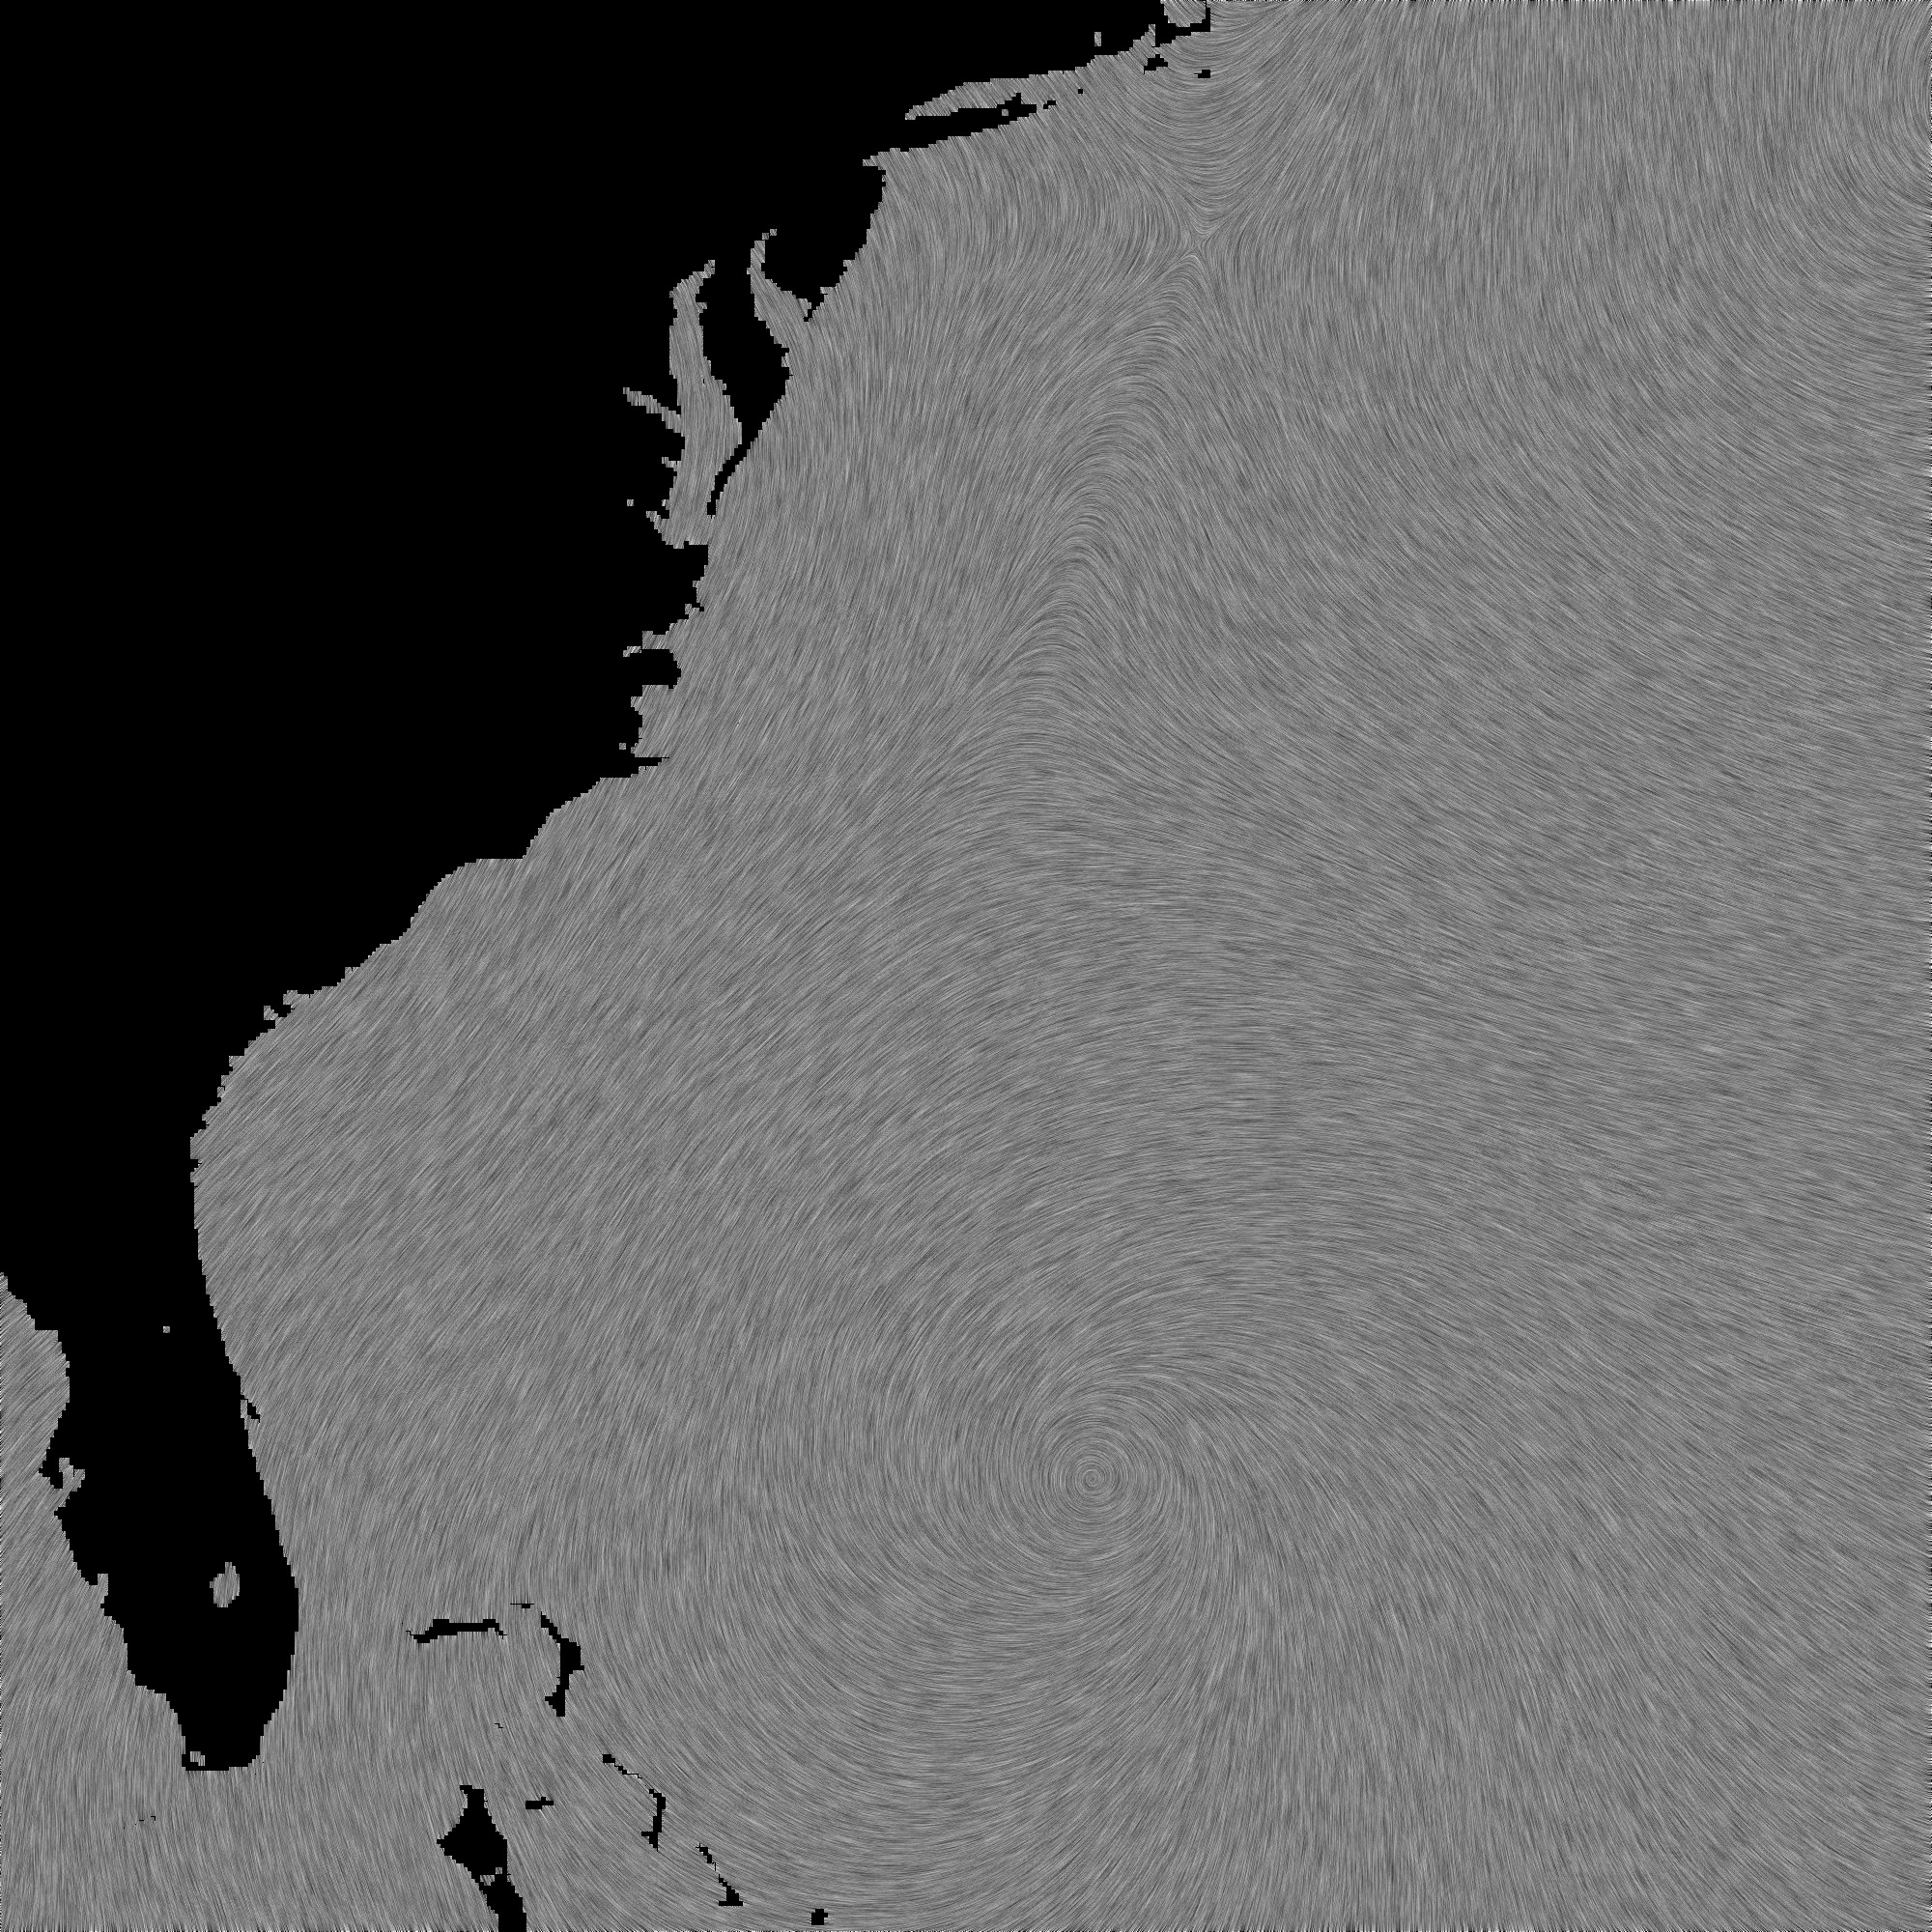
\includegraphics[width=0.7\linewidth]{isabel_linelength_10_highdef.jpg}
 \caption{Isabel set, same gimmick, 5\%}
 \label{fig11}
\end{figure}
\begin{figure}\centering
 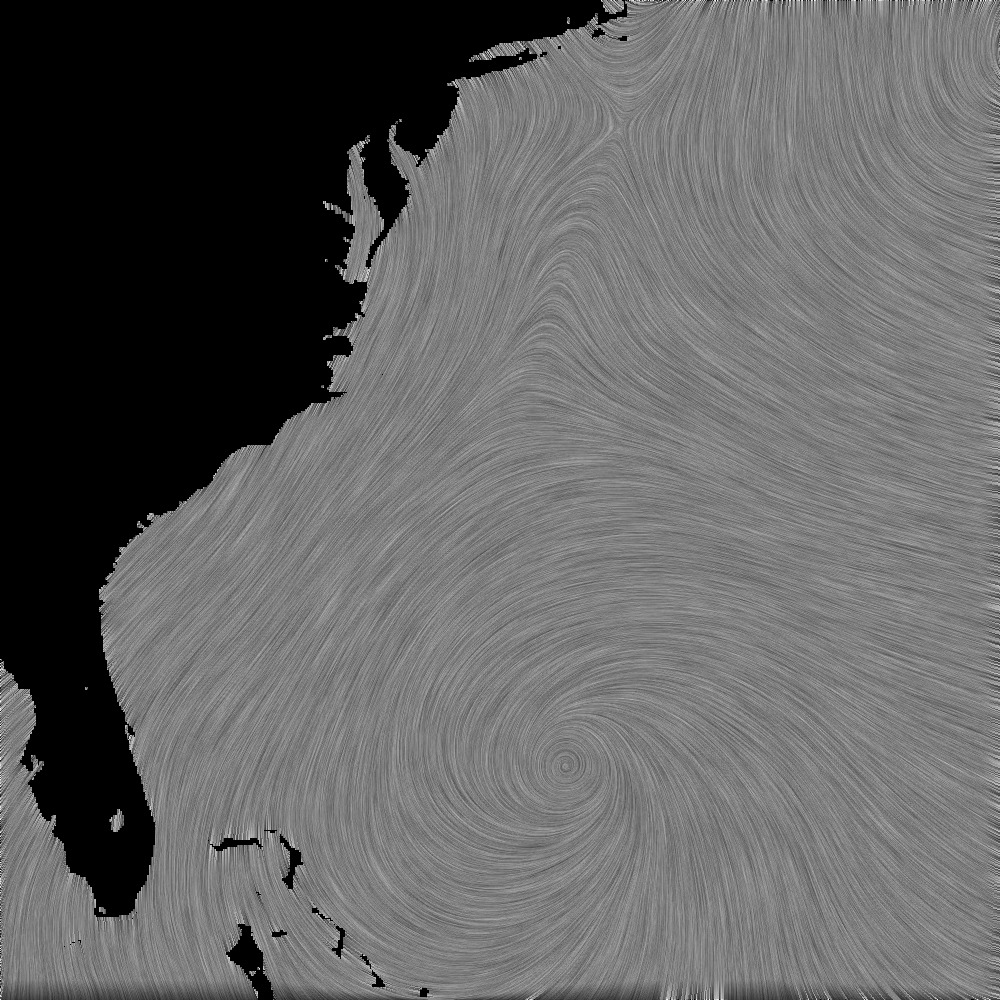
\includegraphics[width=0.7\linewidth]{isabel_linelength_20_highdef.jpg}
 \caption{Medium Lines (10\% of the image width)}
 \label{fig12}
\end{figure}
\begin{figure}\centering
 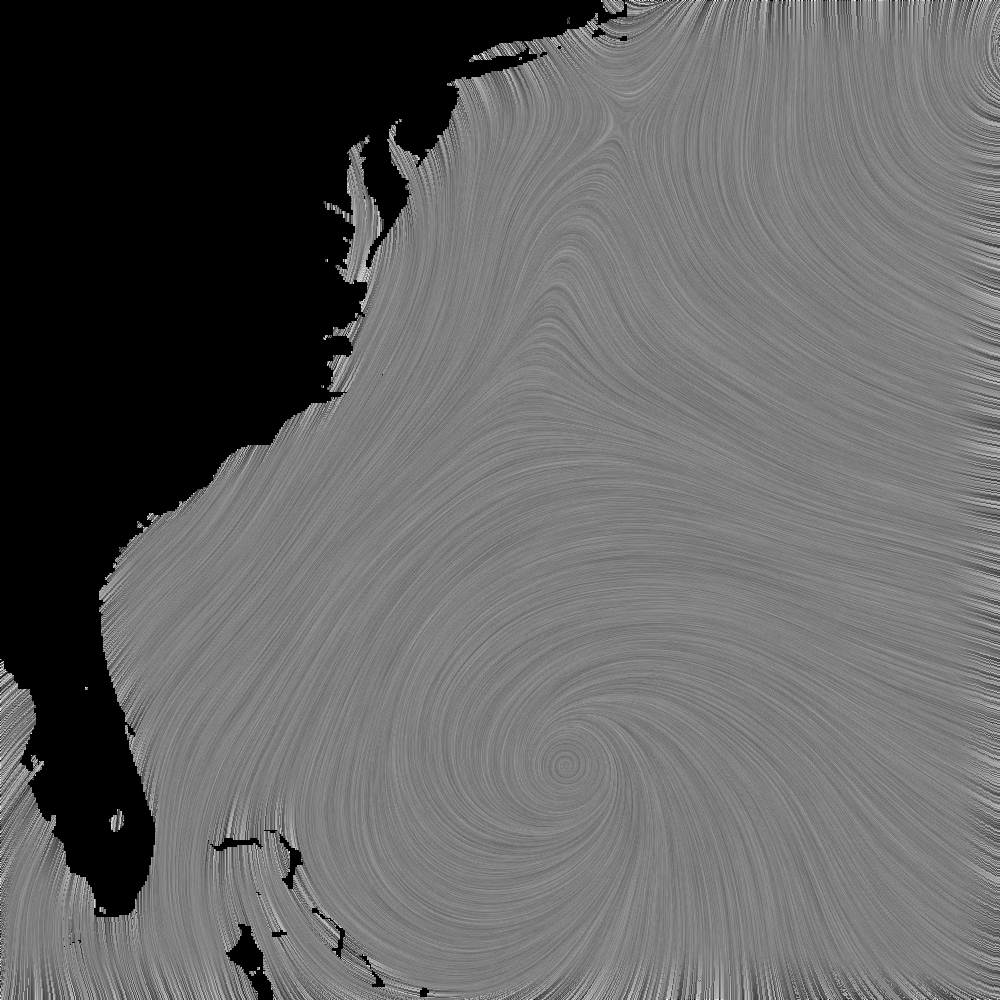
\includegraphics[width=0.7\linewidth]{isabel_linelength_50}
 \caption{Long lines (20\%)}
 \label{fig13}
\end{figure}


\end{document}
